\section{Modèles de programmation à base de tâches}\label{sec:context:others}

Il existe de nombreux modèles de programmation à base de tâches, certaines fonctionnalités diffèrent, mais les concepts de base restent les même, et seront détaillés ci dessous.

\subsection{L'unité de base : la tâche}

Une tâche peut être vue comme la plus petite quantité de travail séquentiel exécutable sur un processeur.
En pratique c'est une section de code bien définie du programme, et cela peut être une simple instruction, un bloc de code délimité, ou encore une fonction très complexe.
La quantité de calcul idéale dans une tâche - la \emph{granularité} - peut varier fortement en fonction de l'application et du support exécutif, ce point est abordé en détail dans la section~\ref{sec:context:others:granularity}

Une tâche est nécessairement accompagnée de données qu'elle manipule. De la même manière qu'une fonction utilise des paramètres, le bloc de code composant une tâche utilise des variables qui peuvent être soit locales (on parlera alors de données privées), soit partagées par d'autres parties du code (on parlera de données partagées).


\subsection{Traitement d'une tâche : de la création à l'exécution}\label{sec:context:others:costs}

Si la notion de tâche peut paraître simple, elle s'accompagne d'un certain nombre de traitements plus ou moins automatiques (en fonction du modèle de programmation), mais qui dans tous les cas ont un coût.
Les trois paragraphes suivants décrivent quelques points clés accompagnant l'utilisation des tâches, qui sont parfois cachés au programmeur.

\subsubsection{Création}

En fonction du modèle de programmation, la création d'une tâche peut être plus ou moins complexe pour le programmeur.

Prenons deux exemples représentatifs pour illustrer.

En StarPU natif, voici par exemple comment on pourrait définir et créer une tâche~:

\begin{lstlisting}[language=c++,caption=Exemple simple en StarPU,label=lst:context:simple-starpu]
void work() {
  // calcul
}

int main() {
  // ...
  struct starpu_codelet dummy_big_cl =
  {
    // ...
    .cpu_funcs = { work },
  };

  task = starpu_task_create();
  task->cl = &dummy_big_cl;
  starpu_task_submit(task);
}
\end{lstlisting}

On voit ici que l'utilisateur doit d'une part avoir isolé la partie calcul de son code, et d'autre part interagir avec le support exécutif de manière significative pour créer une tâche.

Si on regarde maintenant un exemple simple en OpenMP :

\begin{lstlisting}
void foo()
{
  // ...
  int a = 1;
  #pragma omp task shared(a)
  {
    // calcul sur a
  }
  // ...
}
\end{lstlisting}

Cela parait certes moins intrusif et plus simple pour le programmeur, mais pour autant cela ne veut pas dire qu'il y a moins d'actions effectuées en pratique !
Que se passe-t-il vraiment ?

Le compilateur ne va pas laisser ces éléments tels quels dans l'objet binaire généré~: il va les transformer en un ensemble de fonctions élémentaires imposées par le support exécutif. Cet ensemble de fonctions élémentaires s'appelle l'\emph{ABI} (pour \emph{Abstract Binary Interface}).

Un exemple de ce type en OpenMP va donc entrainer deux transformations importantes par le compilateur :
\begin{itemize}
  \item l'\emph{outlining} de la fonction, qui consiste à externaliser le code de la tâche et son contexte dans une fonction séparée.
  \item la substitution du pragma par un appel au support exécutif.
\end{itemize}

Cela donnera au final un code binaire généré correspondant à un programme de ce type, dans l'ABI de Clang :

\begin{lstlisting}
struct unamed_struct_1 {
  int *a;
}

// Outlining du bloc de code correspondant à la tâche
void omp_task_entry(void *args)
{
  struct unamed_struct_1 *shared_variables =
                (struct unamed_struct_1 *) args;
  int a = *(shared_variables->a);
  // calcul sur a
}

void foo()
{
  // ...
  int a = 1;
  // Substitution du pragma par une allocation
  // puis une création de la tâche
  struct unamed_struct_1 tmp;
  tmp.a = &a;
  kmp_task_t task_1 = __kmpc_omp_task_alloc(omp_task_entry, &tmp, /* ... */);

  __kmpc_omp_task(&task_1);
  // ...
}
\end{lstlisting}

Au final les actions effectuées pour la création d'une tâche sont équivalentes, bien que parfois cachées.


\subsubsection{Gestion}

Une fois que le programmeur a défini sa tâche et l'a soumise au support exécutif, celui-ci doit créer et maintenir une structure de données représentant cette tâche.
Celle-ci peut être plus ou moins grande en fonction des informations associées à la tâche.

Le support exécutif va utiliser ces informations au cours de l'exécution du programme pour déterminer quelles tâches sont prêtes pour l'exécution.
En pratique cela signifie que ces structures de données vont être placées dans des conteneurs tels que des files ou des piles, et qu'un certain nombre d'opérations seront effectuées dessus (ajout, suppression, parcours).

En conséquence le coût du maintien des informations à propos d'une tâche entre sa création et son exécution dépend du support exécutif et des structures de données qu'il utilise.


\subsubsection{Exécution}

Cette étape est l'un des points où la gestion par tâche dispose d'un gros avantage par rapport à la création individuelle de threads par le programmeur.
Au début de l'exécution de l'application, un certain nombre de cœurs physiques sont utilisables par le support exécutif (cela peut être déduit implicitement par le support exécutif, ou spécifié explicitement par le programmeur).
Lors de son initialisation, le support exécutif va \textbf{créer et attacher} un thread logique par cœur physique, virtualisant ainsi la gestion des cœurs physiques.

Ces threads vont se voir attribuer différents attributs, comme par exemple une structure de données contenant des tâches.
Ils seront des <<travailleurs>> permanents pour le support exécutif, qui leur donnera des tâches à exécuter au fur et à mesure.

Les threads sont donc les même tout au long de l'exécution de l'application, ce qui évite les coûts liés à la création ou à la destruction de threads. 


\subsection{Moyens de synchronisation}

Lorsqu'on parle de programmation parallèle, il faut bien évidemment parler de synchronisation.
Les différentes tâches définies par l'utilisateur vont être exécutées en parallèle sur la machine, mais dans beaucoup de cas certaines tâches doivent attendre la complétion d'une ou plusieurs tâches avant de pouvoir commencer à être exécutées.

Il y a deux grands types de synchronisations pour la programmation à base de tâches~: la synchronisation explicite, et les dépendances de données.

\subsubsection{Synchronisation explicite}

Le programmeur peut ajouter un point de synchronisation explicite dans le code.
Lorsque le thread exécutant la tâche atteint ce point de synchronisation, il se bloque et attend que l'ensemble des tâches qu'il a créées ait été exécuté avant de reprendre son exécution. Dans l'exemple du listing~\ref{lst:context:task-wait}, exprimé en OpenMP, la tâche C sera garantie d'être exécutée \textbf{après} les tâches A et B.

\begin{lstlisting}[caption=Synchronisation dans le thread courant (OpenMP),label=lst:context:task-wait]
void foo() {
  #pragma omp task
  A();
  #pragma omp task
  B();
  #pragma omp taskwait
  #pragma omp task
  C();
}
\end{lstlisting}


\subsubsection{Dépendances de données}

Le programmeur spécifie des dépendances de données, avec des modes, pour chacune des tâches.
Dans l'exemple du listing~\ref{lst:context:task-dep}, la tâche |write_A| possède une dépendance en \emph{écriture} sur la variable |a|, et la tâche |read_A| possède une dépendance en \emph{lecture}.

Étant donné qu'il y a une lecture et une écriture, le principe de cohérence séquentielle impose que les opérations soient ordonnées dans l'ordre où elles ont été créées (ici la tâche en lecture devrait avoir lieu \textbf{après} la tâche en écriture).

Si on regarde le reste du programme, la tâche |write_B| dispose d'une dépendance en écriture sur |b| et la tâche |read_AB| souhaite lire |a| et |b|.

Étant donné que du point de vue des dépendances les tâches |write_A| et |write_B| sont indépendantes, elles pourraient très bien être exécutées en même temps, et |write_B| pourrait terminer son exécution avant même que |read_A| commence la sienne.

En revanche |read_AB| devra forcément être exécutée après |write_A| et |write_B| puisqu'elle a une dépendance en lecture sur des données écrites par ces deux tâches, et qu'elle a été créée après dans l'ordre séquentiel.


\begin{lstlisting}[caption=Synchronisation via des dépendances (OpenMP),label=lst:context:task-dep]
void foo() {
  int a;
  int b;
  #pragma omp task depend(out: a)
  write_A(&a);
  #pragma omp task depend(in: a)
  read_A(&a);
  #pragma omp task depend(out: b)
  write_B(&b);
  #pragma omp task depend(in: a, b)
  read_AB(a, b);
}
\end{lstlisting}

Cet exemple de code se traduit en un graphe de tâches direct et acyclique (\emph{DAG}) équivalent à la figure~\ref{fig:context:dag-dataflow}, sur lequel apparaissent également les différentes versions des variables.

\begin{figure}[ht]
  \centering
  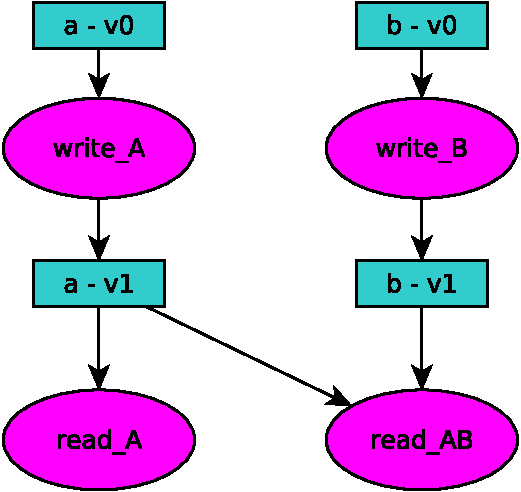
\includegraphics[width=0.5\textwidth]{dataflow-example}
  \caption{DAG équivalent au listing~\ref{lst:context:task-dep}}\label{fig:context:dag-dataflow}
\end{figure}

Les deux types de synchronisation ont des avantages et des inconvénients : la synchronisation dans le thread courant représente très peu d'overhead lors de l'exécution, mais si le travail est légèrement déséquilibré, certains threads pourraient rester inactifs alors que des tâches pourraient être exécutées.
Les dépendances induisent un coût de calcul des tâches prêtes lors de l'exécution, mais maximise l'utilisation des ressources.


\subsection{Quelques exemples de modèles de programmation}

Plusieurs modèles de programmation populaires proposent d'exprimer du parallélisme à base de tâches, parmi lesquels Cilk, TBB, et OpenMP, qui fonctionnent chacun avec des méthodes différentes : respectivement via des annotations sur des fonctions, des appels dans le code utilisateur, et des directives pour le compilateur.

Les listings~\ref{lst:context:cilk},~\ref{lst:context:tbb}, et ~\ref{lst:context:openmp} donnent une comparaison de l'expression du même exemple simple, le calcul du nième nombre de la suite de Fibonacci.

Les modèles de programmation plus spécifiques à certaines constructions ou architectures seront abordés dans la section~\ref{sec:rw:other-runtimes}

\subsubsection{Cilk}

Cilk~\cite{cilk5} est un modèle de programmation basé sur C.
Il introduit principalement deux nouveaux mots clés : |cilk_spawn| et |cilk_sync|, pour, respectivement, exposer du parallélisme et introduire un point de synchronisation.
Le mot clé |cilk_spawn| vient précéder un appel de fonction pour indiquer que la fonction peut s'exécuter en parallèle. Cela en fait donc un modèle de programmation à base de tâches.
Cilk propose également une extension de la notation de tableau, ayant pour but de faciliter la vectorisation automatique par le compilateur.


\begin{lstlisting}[language=c++,caption=Fibonacci exprimé en Cilk,label=lst:context:cilk]
int fib(int n) {
  if (n < 2)
    return n;
  int x = cilk_spawn fib(n-1);
  int y = fib(n-2);
  cilk_sync;
  return x + y;
}
\end{lstlisting}


\subsubsection{Threading Building Block}

Threading Building Block (TBB)~\cite{Reinders2007} est un modèle de programmation développé par Intel comme une bibliothèque C++.

Elle propose différentes fonctions pour que le programmeur puisse exprimer du parallélisme, dont notamment :
\begin{itemize}
  \item La fonction template |parallel_for|, s'appliquant sur une boucle et prenant en paramètre une fonction utilisateur.
    La bibliothèque découpe automatiquement l'espace d'itération en groupes d'itérations et envoie un itérateur C++ à la fonction utilisateur pour son traitement.
  \item Un ensemble de fonctions pour accéder à l'ordonnanceur de tâches de la bibliothèque.
\end{itemize}

La bibliothèque propose également un ensemble de structures de données à accès concurrent (listes, tables de hachage), ainsi que des allocateurs mémoire.

\begin{lstlisting}[language=c++,caption=Fibonacci exprimé en TBB,label=lst:context:tbb]
#include "tbb/task_group.h"
using namespace tbb;

int Fib(int n) {
  if( n<2 ) {
    return n;
  } else {
    int x, y;
    task_group g;
    g.run([&]{x=Fib(n-1);}); // création d'une tâche
    g.run([&]{y=Fib(n-2);}); // création d'une autre tâche
    g.wait();                // synchronisation
    return x+y;
  }
}
\end{lstlisting}

\subsubsection{OpenMP}

OpenMP~\cite{openmp45} est un modèle de programmation supportant le C/C++ et Fortran.
Il s'utilise à travers des directives de compilation ainsi qu'une API, et propose lui aussi les constructions classiques : boucles, tâches, et autres éléments facilitant la programmation parallèle.

Originellement OpenMP ne proposait que du parallélisme de boucle, le concept de tâches n'a été introduit que plus tard avec OpenMP~3.0, et le concept de dépendances de données entre tâches a été introduit encore plus tard avec la version~4.0.

Le standard d'application de nos idées pour cette thèse étant OpenMP, une description détaillée des fonctionnalités et de ses spécificités est faite dans la section~\ref{sec:context:openmp}.

\begin{lstlisting}[language=c++,caption=Fibonacci exprimé en OpenMP,label=lst:context:openmp]
int fib(int n) {
  if (n < 2)
    return n;
#pragma omp task
  int x = fib(n-1);
  int y = fib(n-2);
#pragma omp taskwait
  return x + y;
}
\end{lstlisting}

\subsection{Quantité de travail et granularité}\label{sec:context:others:granularity}


Dans ce type de modèles de programmation, la clé pour maximiser l'utilisation des ressources est de réduire l'overhead du support exécutif par rapport au calcul en trouvant le bon \emph{grain} de tâche.

Il faut donc jouer sur le degré de parallélisme pour atteindre les meilleures performances : les tâches doivent être suffisamment petites pour proposer le maximum de parallélisme, mais pas trop pour ne pas surcharger le support exécutif, vis à vis des coûts décrits dans la section~\ref{sec:context:others:costs}.

Ce grain optimal dépend de plusieurs facteurs : les structures de données utilisées par le support exécutif, le coût de création des tâches, et la quantité de travail mis à disposition par cœur via ce grain.

Cela peut être illustré via une application telle que la factorisation de Cholesky par bloc : à taille de matrice fixée le nombre de tâches créées dépend directement de la taille de bloc choisie.
Plus la taille de bloc est petite, plus le nombre de blocs créés (et donc le nombre de tâches, et le parallélisme potentiel) est important.

\begin{figure}[ht]
  \centering
  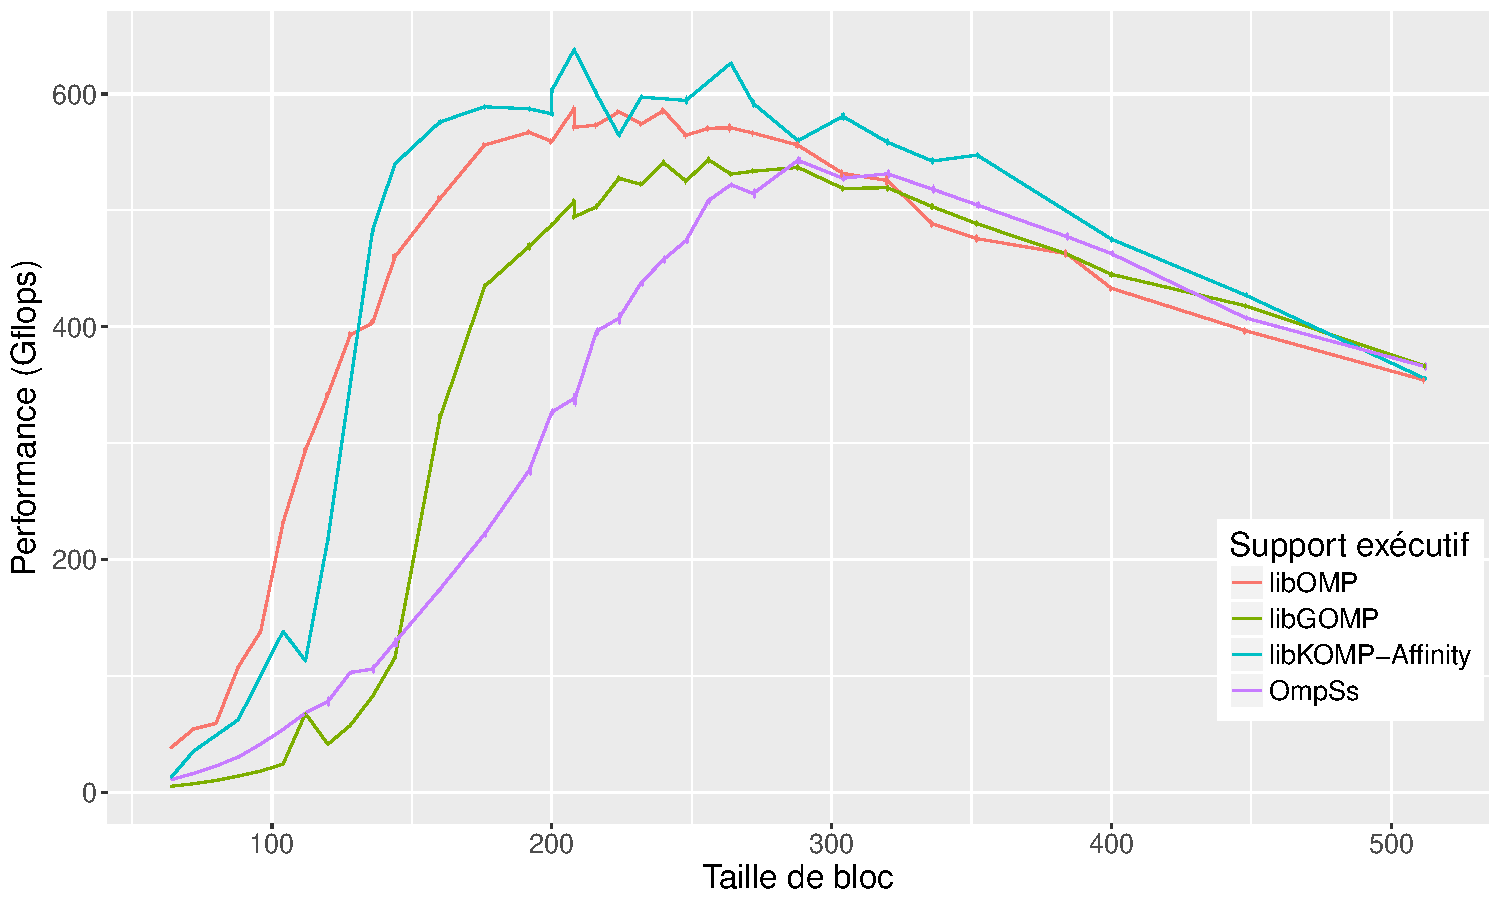
\includegraphics[width=0.92\textwidth]{graph_granularity_8k_64.pdf}
  \caption{Performances de Cholesky pour une matrice de taille 8192 et 64 threads, en fonction de la taille de bloc}\label{fig:context:granularity}
\end{figure}

La figure~\ref{fig:context:granularity} illustre l'évolution des performances d'une factorisation de Cholesky d'une matrice de taille 8192, sur un nombre de cœurs fixé (64), en fonction de la taille de bloc et du support exécutif.
Comme on peut le voir, les parties extrèmes de la courbe se comportent de manière similaires quel que soit le support exécutif : une taille de bloc trop faible génère beaucoup trop de tâches et les support exécutifs sont complètement surchargés. Une taille de bloc trop importante limite complètement le parallélisme et donc les performances.

\begin{todo}
  @Thierry : revoir la courbe, en particulier quels runtimes affichés ?

  Ici c'est la première fois qu'on parle d'ompss et libkomp, on peut ne parler que des trucs standards et ressortir dans une section éval de perf.

  Ou faire un paragraphe de blabla rapide sur ompss et libkomp, en disant qu'on en parlera plus tard
\end{todo}

Le grain adapté n'est pas nécessairement unique : en fonction du support exécutif on peut avoir un choix plus ou moins important. Cela est illustré sur la figure~\ref{fig:context:granularity} : avec OmpSs le grain optimal se situe dans un intervalle de tailles de blocs assez restreint (entre environ 250 et 350), alors qu'avec clang ou libkomp une taille de bloc entre 150 et 350 permet d'obtenir des performances sensiblement équivalentes.

La courbe tracée avec libkomp inclut nos travaux sur l'affinité, et permet d'illustrer que même si l'affinité permet d'influer sur les performances maximales, elle n'a pas vraiment d'impact sur le grain optimal, comme cela est illustré sur la figure~\ref{fig:context:granularity-16k}, ou le maximum de performance est obtenu pour tous les supports exécutifs aux environs de 300.


\begin{figure}[ht]
  \centering
  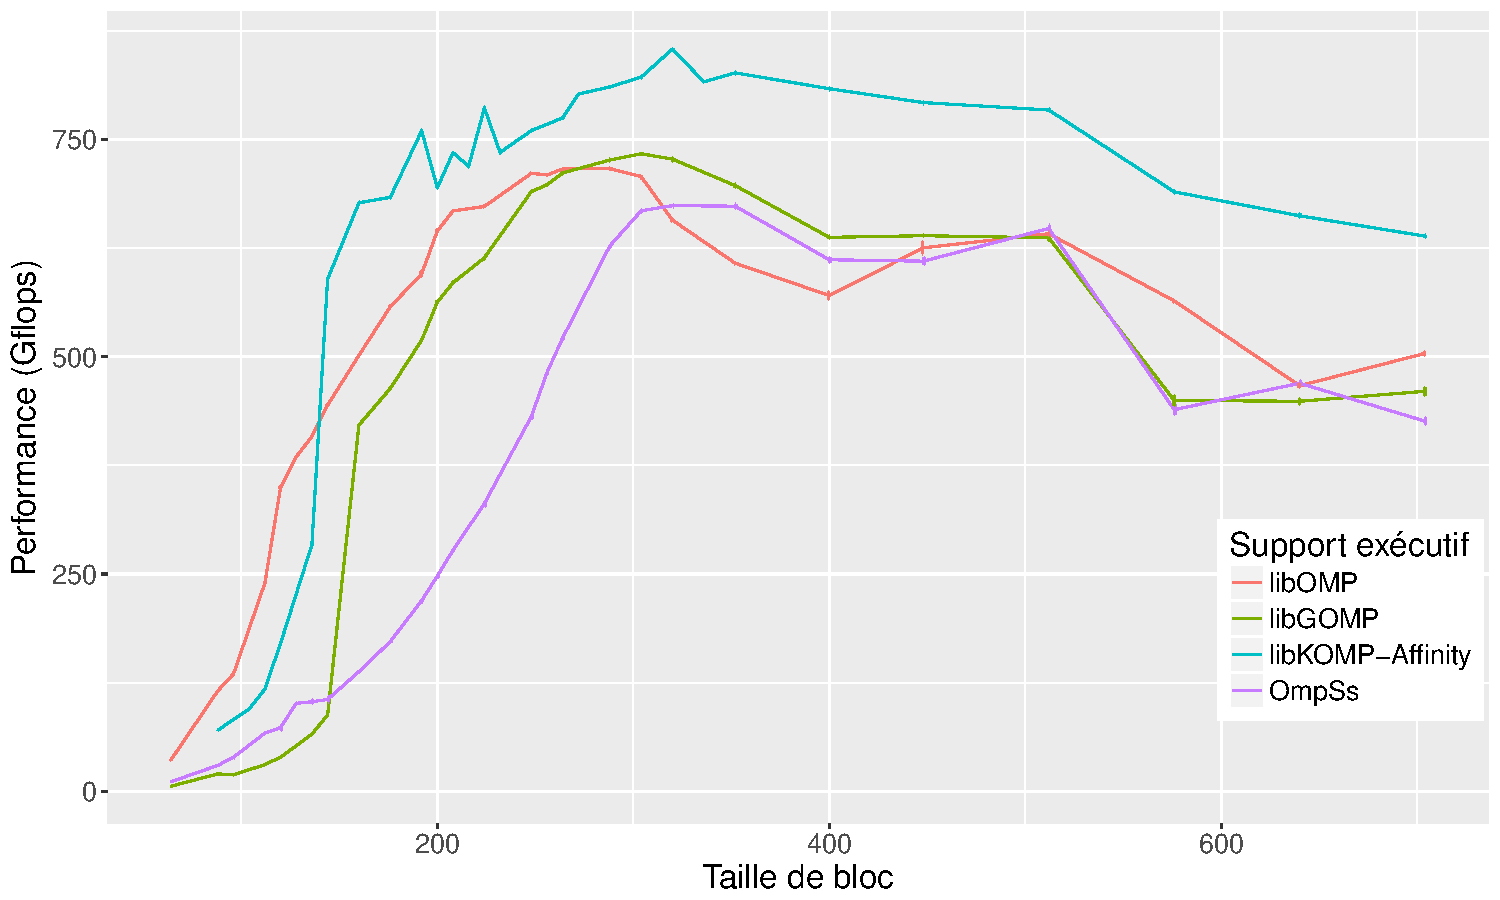
\includegraphics[width=0.92\textwidth]{graph_granularity_16k_64.pdf}
  \caption{Performances de Cholesky pour une matrice de taille 163384 et 64 threads, en fonction de la taille de bloc}\label{fig:context:granularity-16k}
\end{figure}


Le choix du grain pour une tâche dépend entièrement de l'application, et reste à l'appréciation du programmeur.

\bigskip

Bien que tous ces modèles de programmation aient leur spécificités, ils permettent tous de décrire l'application sous forme de graphe de tâches direct et acyclique (DAG).

L'étape suivante consiste à exécuter ce graphe sur la machine, et pour cela le support exécutif peut se reposer sur un ensemble important de techniques d'ordonnancement. 


